%
% string.tex -- vibrating string
%
% (c) 2019 Prof Dr Andreas Müller, Hochschule Rapperswil
%
\documentclass[tikz,12pt]{standalone}
\usepackage{amsmath}
\usepackage{times}
\usepackage{txfonts}
\usepackage{pgfplots}
\usepackage{csvsimple}
\usetikzlibrary{arrows,intersections,math,hobby}
\begin{document}
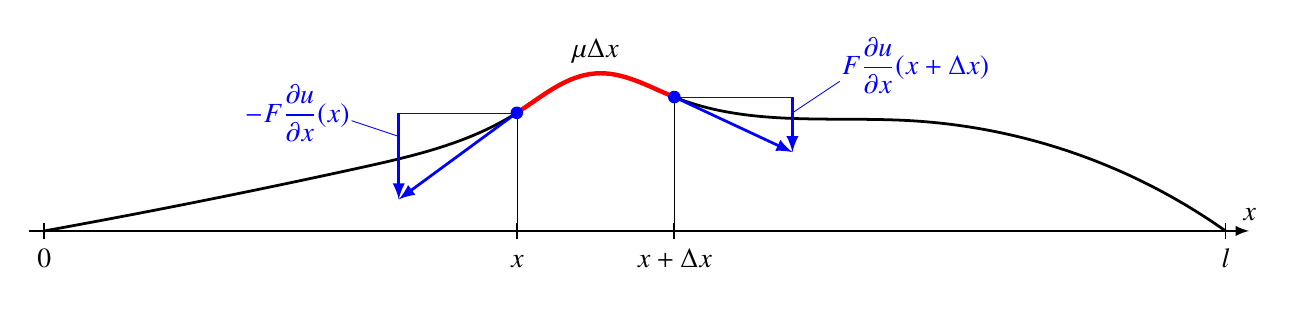
\begin{tikzpicture}[>=latex,use Hobby shortcut]

\draw[->,line width=0.7pt] (-0.2,0)--(15.3,0) coordinate[label={$x$}];
\draw[line width=0.7pt] (0,-0.1)--(0,0.1);
\draw[line width=0.7pt] (15,-0.1)--(15,0.1);

\coordinate (A) at (0,0);
\coordinate (B) at (15,0);

\coordinate (C05) at (4,0.8);
\coordinate (C10) at (6.0,1.5);
\coordinate (C20) at (7,2);
\coordinate (C30) at (8.0,1.7);
\coordinate (C40) at (11,1.4);

\node at (0,-0.1) [below] {$0\mathstrut$};
\node at (15,-0.1) [below] {$l\mathstrut$};

\draw[line width=1pt] (A) .. (C05) .. (C10) .. (C20) .. (C30) .. (C40) .. (B);
\begin{scope}
\clip (6,0) rectangle (8,2.1);
\draw[line width=1.6pt,color=red] (A) .. (C05) .. (C10) .. (C20) .. (C30) .. (C40) .. (B);
\end{scope}

\draw[->,line width=1pt,color=blue] (C10)--(4.5,0.4);
\draw[->,line width=1pt,color=blue] (C30)--(9.5,1.0);

\draw[line width=0.1pt] (6,0)--(C10);
\draw[line width=0.1pt] (8,0)--(C30);

\draw[line width=0.7pt] (6,-0.1)--(6,0.1);
\draw[line width=0.7pt] (8,-0.1)--(8,0.1);

\node at (6,-0.1) [below] {$x\mathstrut$};
\node at (8,-0.1) [below] {$x+\Delta x\mathstrut$};

\draw[color=blue,line width=0.1pt] (C10)--(4.5,1.5);
\draw[->,color=blue,line width=1pt] (4.5,1.5)--(4.5,0.4);
\draw[color=blue,line width=0.1pt] (C30)--(9.5,1.7);
\draw[->,color=blue,line width=1pt] (9.5,1.7)--(9.5,1.0);

\node[color=blue] at (10,2.1)
	[right]  {$\displaystyle F\frac{\partial u}{\partial x}(x+\Delta x)$};
\draw[color=blue,line width=0.3pt] (10.1,1.9)--(9.5,1.5);
\node[color=blue] at (4,1.5)
	[left] {$\displaystyle -F\frac{\partial u}{\partial x}(x)$};
\draw[color=blue,line width=0.3pt] (4.5,1.2)--(3.9,1.4);

%\fill[color=blue] (C05) circle[radius=0.08];
\fill[color=blue] (C10) circle[radius=0.08];
%\fill[color=blue] (C20) circle[radius=0.08];
\fill[color=blue] (C30) circle[radius=0.08];
%\fill[color=blue] (C40) circle[radius=0.08];

\node at (C20) [above] {$\mu \Delta x$};

\end{tikzpicture}
\end{document}

